\subsubsection{Spoof Access Point}
\label{sec:spoofap}
This is not necessarily an attack in itself, but a means of relying on social engineering to gain connections to perform attacks on. A soft access point is a rogue access point that has been established on a wireless adaptor, without the need for a router. Leaving this open, and performing in an area with a high footfall or cafe area, will allow the attacker to gain connections, monitor traffic, and perform various man-in-the-middle attacks. It can also be paired with other attacks detailed further on in the report.

\begin{figure}[h!]
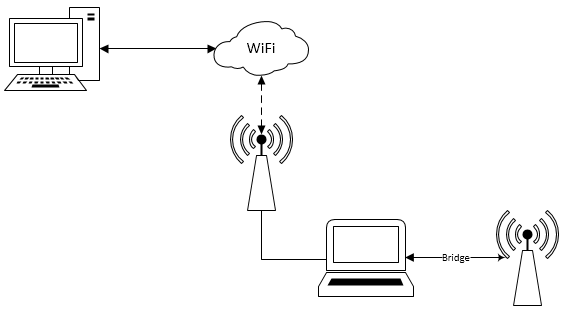
\includegraphics[width=\linewidth]{research/figures/spoofap.png}
\caption{Soft access point bridges traffic to real access point.}
\end{figure}

\subsubsection*{Performing the Attack}
As this is more of a gateway attack, not a lot can be gained from doing it alone. The airbase-ng tool proved the simplest way to create a fake access point, taking the wireless interface and start/stop as parameters. The image below shows the creation of an access point and a station connecting to it. The access point then bridges it’s traffic to an actual network connection in order for the station to access the internet and the attacker to monitor passing traffic.

\begin{figure}[h!]
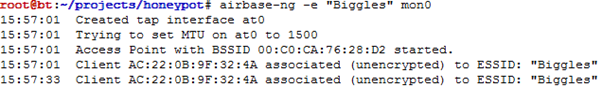
\includegraphics[width=\linewidth]{research/attackvectors/figures/spoofap1.png}
\caption{Soft access point created with the SSID “Biggles”.}
\end{figure}